% \chapter{Pr\'ologo}
%
Estas notas de curso est\'an dise\~nadas para guiar al estudiante universitario que, por primera vez, se encuentra cara a cara contra los diversos temas vistos en un curso normal de F\'isica 1. Dichos temas abarcar\'an las \'areas de mec\'anica, an\'alisis vectorial, trabajo, energ\'ia y fluidos, entre otros. 

Se espera que el estudiante tenga buen manejo del \'algebra, as\'i como de an\'alisis gr\'afico, num\'erico y geom\'etrico, pero tambi\'en se espera que el estudiante los desarrolle y se mejore al mismo tiempo a lo largo del curso.

\section{Composici\'on del Curso}

Primero lo primero: las notas. Si bien el programa del curso es bien detallado, hay algo muy sensible a dejar claro desde el inicio: \textbf{no habr\'an puntos extras, bajo ning\'un motivo}. La mayor\'ia de la nota ($57\%$) vendr\'a de los tres ex\'amenes parciales y ex\'amen final, valiendo 14 puntos cada parcial y 15 puntos el final. Habr\'an dos revisiones de sus notas de clase, i.e. de su cuaderno, por lo que se sugiere que lo tengan consigo tanto para las clases te\'oricas como para los laboratorios.

A lo largo del curso, habr\'an comprensiones de lectura, o Gu\'ias de Comprensi\'on Lectora (GCL). \'Estas se les entregar\'an

Las tareas/hojas de trabajo les ser\'an entregadas tanto en forma f\'isica como en forma digital, ya sea enviadas por correo o subidas a Canvas. Todos los documentos, incluidas estas notas de curso, ser\'an subidas y actualizadas con frecuencia a Canvas, as\'i que se le pide al alumno que revise con frecuencia \'este medio. Es posible que algunas tareas consistan en que el estudiante revise su propia tarea, siempre que se le proporcione el solucionario con anticipaci\'on. De ser as\'i, la nota consistir\'a en llenar un formulario en Google Forms (el link ser\'a proporcionado via un correo electr\'onico), as\'i como la entrega de la tarea en forma f\'isica. Se proporcionar\'a el solucionario y el estudiante, al llenar el formulario de Google Forms, reflexionar\'a si tuvo o no alg\'un problema y si tiene dudas persistentes. Se espera que el estudiante sea honesto y escriba cualquier duda que tenga, con el fin de ayudarlo a entender el tema lo antes y de la mejor manera posible.

En la semana de clases previa a cada ex\'amen parcial habr\'a un respectivo simulacro. Dicho simulacro consistir\'a en un per\'iodo de clase dedicado a resolver preguntas del mismo nivel que los parciales, y en el siguiente per\'iodo se har\'a la resoluci\'on de los mismos. La nota de los primeros dos simulacros ser\'a dividida en $50\%$ para la correcci\'on de los ejercicios, y $50\%$ para la reflexi\'on de los errores cometidos. Para el \'ultimo simulacro, la nota ser\'a $100\%$ en la reflexi\'on de los errores.

Los laboratorios ser\'an los viernes de $7:00$ a.m. a $9:25$ a.m. en el C-115. Debido a que existen 5 minutos de descanso entre per\'iodo, se juntar\'an \'estos al final para as\'i salir 10 minutos antes, es decir, a las $9:15$ a.m., para evitar cualquier confusi\'on.

Debido a pol\'iticas internas del departamento de F\'isica, los auxiliares \textbf{NO} podr\'an responder un correo que est\'e dirigido a ellos \'unicamente. Si desean una respuesta a una consulta hecha v\'ia correo electr\'onico, toda conversaci\'on deber\'a de enviarse con copia a mi correo. \'Esto es para prevenir cualquier malentendido y asegurarse que todas las partes est\'en enteradas de cualquiera que sea la duda.

\paragraph{Libro de texto: Serway \& Jewett, \textit{F\'isica para ciencias e ingenier\'ia}, 10a edici\'on, Vol. 1, 2017}

\begin{center}
    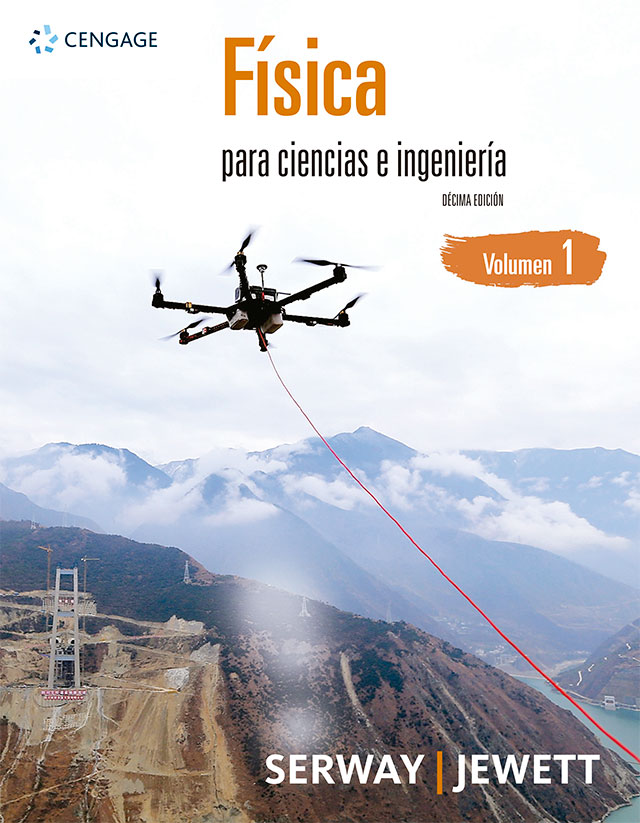
\includegraphics[width=0.65\textwidth]{serwayjewett.JPG}
\end{center}

\newpage